\chapter{Postprocessing: The visualisation toolkit, IO and \Peano\
scripts}
\label{chapter:postprocessing}



We do offer three different ways to handle \Peano\ output, i.e.~the native Peano
patch files:

\begin{enumerate}
  \item You visualise them directly within Paraview (Section~\ref{label:postprocessing:display-in-paraview}).
  \item You use a Python-based visualisation suite from the command line. The steps 
  are the same as in Section~\ref{label:postprocessing:display-in-paraview}.
  \item You convert the patch files via a C++ command line tool into VTK and
  postprocess the data from there
  (Section~\ref{section:postprocessing:command-line}).
\end{enumerate}


\noindent
The following three sections discuss these three routes, before I give some
general visualisation comments in
Section~\ref{section:postprocessing:tweaking-pictures}. 
Furthermore, I sketch further Python scripts that can be used to postprocess
some output you get from any \Peano\ application.
This is information about the general runtime or load balancing distribution,
e.g.


\section{Displaying \Peano\ files directly within Paraview}
\label{label:postprocessing:display-in-paraview}

\begin{remark}
  \Peano's postprocessing scripts use Python 3. This means you need a Paraview
  version with Python 3 support (oldish Paraview installations only support
  Python 2.7, and some Paraview downloads don't come along with Python support
  at al).
\end{remark}


\noindent
You can display \Peano's patch files directly within Paraview. 
Again, there are different ways.
For all of them, \Peano's Python environment has to be available within Paraview:



\paragraph{Prepare system.}
%
%
Before you start up Paraview, ensure that both the \Peano\ \texttt{python}
directory and any third-party Python lib are in your path. 
On some systems, Paraview seems to
only know its internal libraries, so you have to add these manually. On my
system, I use
  \begin{code}
export PYTHONPATH=../../../python:/usr/lib/python3/dist-packages  
  \end{code}
The latter holds \texttt{jinja2} on my system.


\paragraph{Start Paraview's Python environment.}
%
%
You can either manipulate all data directly within Paraview or use Paraview's Python 
terminal to convert data as a batch from Peano's native format into native Paraview data.
I recommend the direct Paraview terminal route to interactively explore data.
The actual data processing (of time-dependent data) however can be very slow.
Once I know what information I need, I thus usually switch to Paraview's Python interpreter 
to convert all data into Paraview's native file formats in one rush.


\begin{center}
 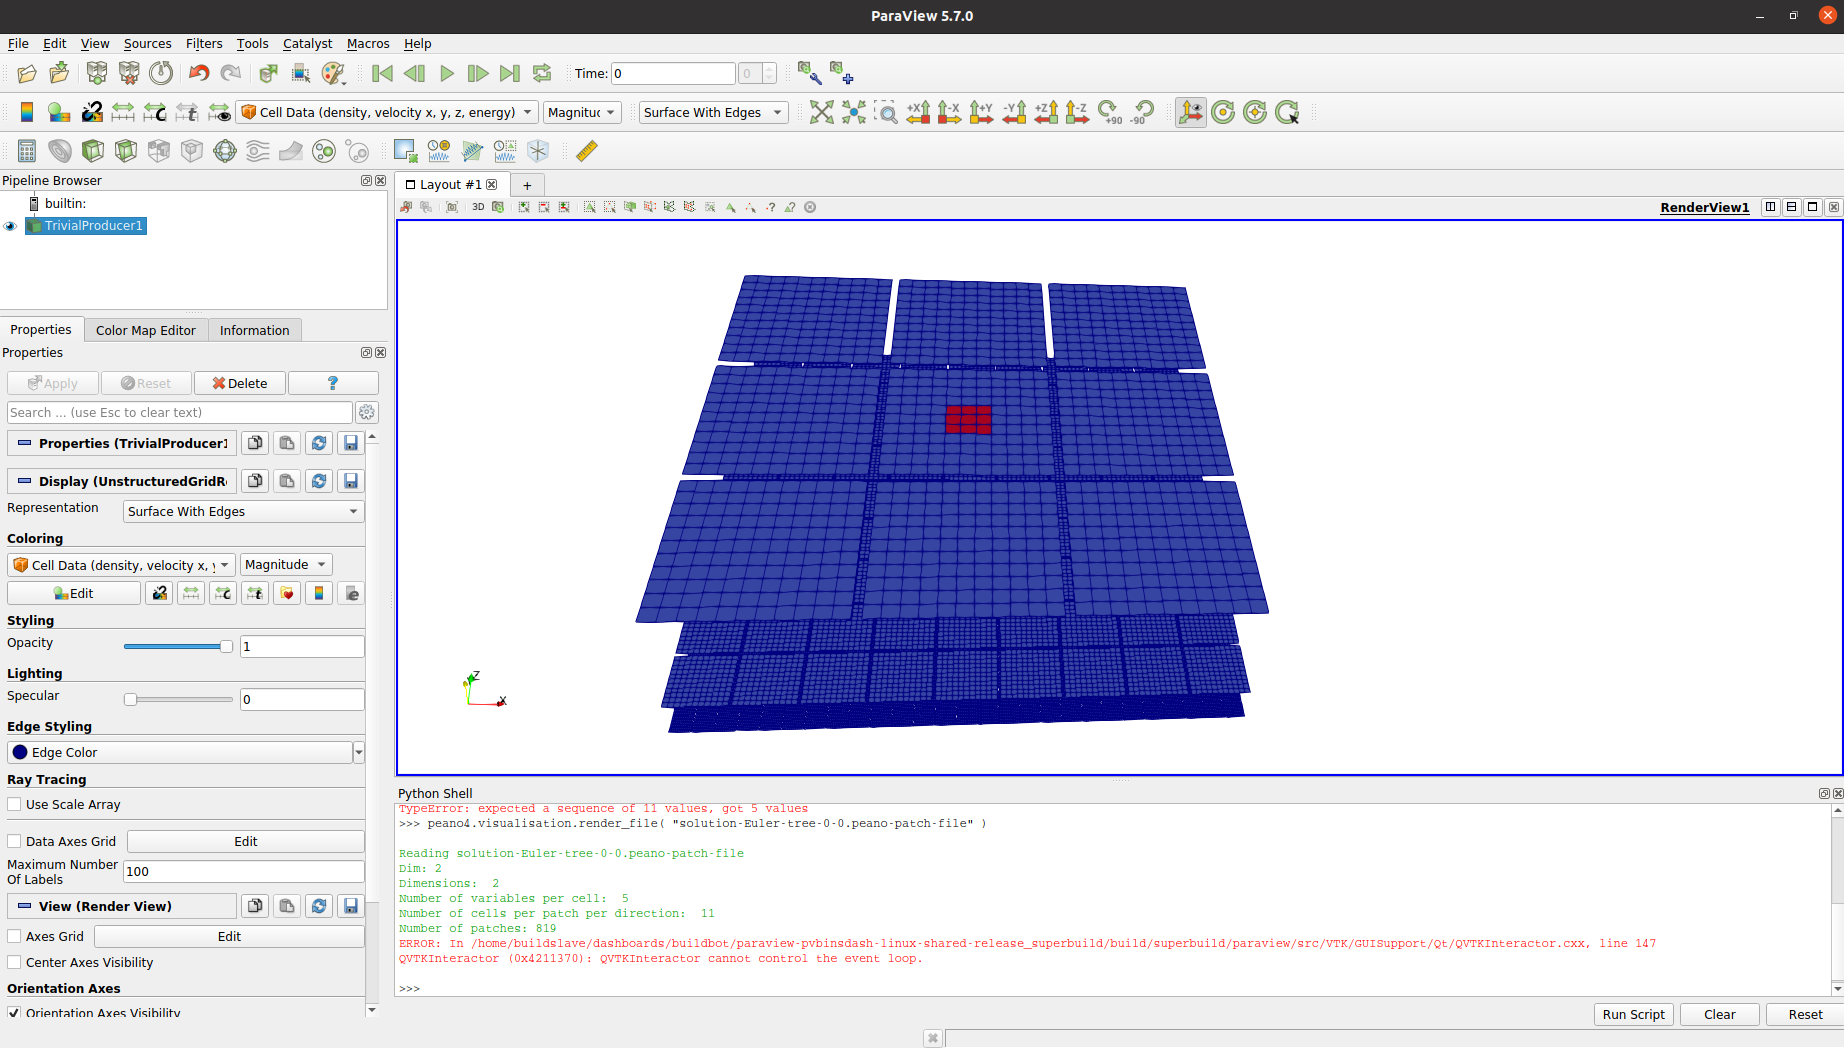
\includegraphics[width=0.6\textwidth]{80_postprocessing/paraview.png}
\end{center}


For the batch mode, open the terminal \texttt{pvpython}.
For the interactive GUI mode, open Paraview and activate the Python Shell by clicking the check box in
the View menu.


Both visualisation routes first require you to load \Peano's Python tools---either
within the \texttt{pvpython} terminal or the Paraview Python window:
\begin{code}
import peano4.visualisation  
\end{code}


\paragraph{Work with a whole dataset.}
%
%
%
\Peano\ provides a Python class \texttt{Visualiser} which allows you to navigate through the whole data:
\begin{code}
import peano4.visualisation
visualiser = peano4.visualisation.Visualiser( "solution-Euler.peano-patch-file" )
visualiser.display()
visualiser.append_filter(peano4.visualisation.ExtractFineGridFilter())
\end{code}

\noindent
The snippet displays the first dataset (time step) from a \Peano\ data dump.
Via 
\begin{code}
visualiser.select_dataset(10)
visualiser.reload()
\end{code}
you can, for example, select the 11th data set and display this one.


Running through data sets (time steps) manually is cumbersome in many cases.
We have not yet managed to integrate our Python-based, bespoke postprocessing
into Paraview's video replay features, and we also experience that it is relatively 
slow.
In such a case, it is more convenient to convert all data in one rush 
into Paraview's native, binary file format vtu:
\begin{code}
visualiser.write_vtu_time_series()
\end{code}


\noindent
Once this routine terminates, you'll find a file with the extension \texttt{.pvd}
in your directory which you can open and play as video.
Obviously, this conversion can be triggered in Paraview's Python interpreter 
which is typically faster than Paraview's built-in terminal.

\begin{remark}
 You can trigger the Python postprocessing routines while the simulation is running.
\end{remark}



\paragraph{Display a single file.}
%
%
Load the file you are interested in via
\begin{code}
data = peano4.visualisation.render_single_file(  "solution-Euler-tree-0-0.peano-patch-file", identifier="MyQName" )
\end{code}

\noindent
This is only one snapshot file, i.e.~one file written by one thread in one step. 
We can display the file with
\begin{code}
tp = TrivialProducer()
tp.GetClientSideObject().SetOutput(data)
Show(tp)
\end{code}


\noindent
If we write large parallel files or time series, \Peano\ will typically 
create one file like \texttt{solution-Euler.peano-patch-file} which links
to all the files such as \linebreak \texttt{solution-Euler-tree-0-0.peano-patch-file}.
The meta file (with the links) is plain text, so you can study it via a 
text editor.
Instead of picking a particular file, 
you can display a particular data set (snapshot) from the meta file:
\begin{code}
import peano4.visualisation  
data = peano4.visualisation.render_dataset( \
  "solution-Euler.peano-patch-file", \
  display_as_tree=False, \
  filter=[peano4.visualisation.ExtractFineGridFilter()], \
  dataset_number=0, identifier="MyQName" \
)
tp = TrivialProducer()
tp.GetClientSideObject().SetOutput(data)
Show(tp)
\end{code}


\paragraph{Filters.}
%
%
%
\Peano's data are relatively complex.
In practice, you typically want to filter data before you pipe it into Paraview.
The most popular filter is the one which eliminates the coarse grid levels:
\Peano\ holds all data in multiple resolution.
If your code does not exploit this feature, you might not be interested in the 
coarser resolutions, so removing it makes sense.


There are more filters or you can write your own custom filters.
Study the source code for further details.



\section{Offline/command-line conversion}
\label{section:postprocessing:command-line}


Installing \Peano's VTK command line tools can be quite tricky---depending on your
local VTK installation.
At the same time, the command line conversion via executables, i.e.~not via the 
Python terminal as discussed above, is by far the fastest route.
It  can even exploit multiple cores.
I recommend to stick to the Python-based postprocessing route as long as possible 
and to switch to the offline postprocessing only for large-scale production data
where Python is just too slow and/or all postprocessing has to happen on a remote 
supercomputer as you cannot transfer the (raw) \Peano\ data files.


\begin{remark}
  If you configure \Peano\ with VTK support, \Peano\ builds a command-line tool
  \texttt{convert} which you can use to convert \Peano 's patch files into plain
  (binary) vtk.
\end{remark}



\noindent
Installing VTK support can be challenging. 
Here's some things you might want to consider/check:

\begin{itemize}
  \item To build the \Peano\ conversion/visualisation tools, you have to
  translate the code with \texttt{--with-vtk}. If you don't
  specify a path, then \Peano\ assumes that all VTK is installed 
  within \texttt{/usr/include}\footnote{Recent Ubuntu
  versions for example tend to place VTK in subdirectories of
  \texttt{/usr/local/include}, while SUSE et al indeed place them directly
  within \texttt{/usr/include}. In any case, you will have to select a
  subdirectory from these folders, as VTK usually goes into separate subfolder (depending on their
  version). If you have not installed VTK as stand-alone but as part of the
  Paraview developer version, e.g., then you have to search for the VTK
  directory within the Paraview folder. In any case, search for a
  filte \texttt{vtkVersion.h}. It is the folder hosting this file that we are
  searching for here.}.
  \item We next have to know which VTK version you are using. VTK builds a
  different set of libraries in each generation. \Peano\ has to know which
  version you want to use to link against the right set of libraries. The
  installation script will automatically try to detect your version, but the
  detection is not very robust. If it is the wrong version, use the
  \texttt{--with-vtk-version=x} switch to set the version manually. We currently
  support \texttt{x} 7,8,9, i.e.~we are only interested in the major version of
  your VTK installation. If you have version 8.90, it is the 8 we are interested
  in.
  \item Next, the script will search for the right libraries. By default, our
  script assumes that the libraries are have a suffix with the major dot minor
  number. So we assume that the VTK version 8.90 yields a library
  \texttt{vtkIOCore-8.90}. This is the default. The script will try to find this
  default library and give you some feedback (be careful: if it doesn't find
  the library, it will still continue as you might want to change the pathes
  later on). If your library naming convention is different---we've seen
  systems dropping the version numbers or Paraview installations which append
  something alike \texttt{pv8.90}---then specify your suffix manually through
  \texttt{--with-vtk-suffix}. If your installation does not have a version suffix,
  as is the case in Fedora, you should pass an empty string to this:
  \texttt{--with-vtk-suffix=''}
  \item If your compile passes through but fails in the linking state (object
  not found), then you have to check if the VTK libraries are in the search
  path. If they are not (very likely), then add them prior to the compile call:
\begin{code}
export LDFLAGS="-L/opt/vtk/lib64"
\end{code}
\end{itemize}


\noindent
Once you have managed to configure with VTK and the build process has terminated
successfully, your directory \texttt{src/convert} holds the actual \texttt{convert}
script.
If you call \texttt{convert} without arguments, you get a usage message.
\texttt{convert} allows you to extract data from a data dump, and store it
within the patch files under a new identifier.
It also allows you to extract a dataset from patch files into vtu.
vtu is one of VTK's binary file formats.


A standard postprocessing workflow on the command line reads as follows:
\begin{enumerate}
  \item Use \texttt{convert} to extract certain data from the dumped data files.
  You might want to extract only the finest grid level, e.g., or to pick a
  particular unknown. \texttt{convert} is given a new identifier (name) for the
  new tdata set, and it stores the extracted data either within the existing
  patch files or a new, separate one.
  \item Use \texttt{convert} to pick one particular dataset via its identifier
  and to dump it into a vtu file.
  \item Use Paraview or VisIt to display the vtu file.
\end{enumerate}

%   \item If you configure with \texttt{--with-vtk}, but the makefile cannot find
%   the headers, you have to add the correct search path\footnote.
%   You can either set the
% \begin{code}
% export CPLUS_INCLUDE_PATH=$CPLUS_INCLUDE_PATH:/usr/include/vtk
% \end{code}
%   or you set the corresponding environment variable prior to the configure
%   script. I always recommend that latter route, as our Python API inherits all of the configure
%   variables, i.e.~it will then know where to search for VTK:
% \begin{code}
% export CXXFLAGS=$CXXFLAGS:"-I/usr/local/include/vtk-8.90"
% \end{code}
%   The first setting btw stems from a Fedora system, the latter example from an
%   Ubuntu installation, while OpenSUSE in our test farm got the includes
%   automatically right.


%  Depending on the version chosen, \Peano\ will try to link against a different
%  set of library files.
    
% -with-vtk-version=


  
  
  
  
%   Many VTK installations append the version number to the library, i.e.~they create a library \texttt{libvtkCommonCore-8.90.so} instead of
%   \texttt{libvtkCommonCore.so} if you use VTK 8.9. 
%   \Peano tries to detect this version number automatically but in case it fails,
%   you can use the options \texttt{--with-vtk=<path>} and \texttt{--with-vtk-version=<MAJOR.MINORS>}
%   to specify exactly the Peano version you want to use.
%   If you are not sure, run \texttt{find / -name libvtk*.so} and see what it finds. 
%   %After that, tell the
%   %configuration explicitly which VTK extension to use:
%   %\begin{code}
%   %--with-vtk-version=8.90
%   %\end{code}
%   BTW: Not all Linux distributions install VTK with these extensions, so you
%   have to check manually on your system.

    
\section{Tweaking your pictures}
\label{section:postprocessing:tweaking-pictures}


Peano's default VTK plotters project Peano's tree-based grid onto an
unstructured mesh, as VTK does not support tree meshes.
The underlying mechanism is straightforward:

\begin{enumerate}
  \item If a vertex is touched/read the first time, it is dumped as vertex of
  the unstructured output mesh if it is not refined, i.e.~if no other vertex
  does exist at the same location on a finer mesh level.
  \item If a hanging vertex is created, we add a new vertex to the output dump
  if this hanging vertex has not been written before. The plotters typically
  maintain one big hash map to bookkeep which hanging vertices have already been
  written.
  \item If the tree traversal runs into an unrefined cell, this cell is made a
  cell of the unstructured output mesh.
\end{enumerate}


The block format/the conversion tools in contrast generate all the points
multiple times.
If you have to cells sharing a vertex, the vertex is dumped twice.
For patch-based problems, this is okish, as the number of vertices that are
shared is way smaller than the total number of vertices in the domain (vertices
within a patch are not dumped multiple times).
As a consequence of the redundant vertex dumps, isosurfaces, e.g., might not
work.
If you need them, it is reasonable to project/map the actual data onto a regular
mesh first.


If your PDE has $m$ quantities, Peano's block format dumps them into a vector of
cardinality $m$ per vertex or cell, respectively. 
Most visualisation filters/tools however require data to be either scalar or 
vector data. 
In Paraview, use the calculator filter to extract only some quantities from the 
data dump.
Alternatively, you can ask the convert tool to extract only some data into the
vtu output.

\noindent
Please note that most visualisation codes (such as Paraview) do interpolate
bi-/tri-linearly within the cells. 
If a cell's face is adjacent to cells on finer levels, hanging vertices on the
face exist.
If they do not hold the linearly interpolated value, you will discover
visualisation artifacts.

\begin{remark}
  For smooth output pictures of meshes with adaptivity, you have to 
  \begin{itemize}
    \item set the plotted properties on hanging vertices due to $d$-linear
    interpolation, and
    \item you have to add the plotter mapping after you have invoked the mapping
    that does initialise the hanging vertices.
  \end{itemize}
\end{remark}


\noindent
Please note that the dumped unstructured mesh is a non-conformal mesh. 
Algorithms such as isosurface identification thus might yield invalid
results---it depends on your visualisation algorithms.


% \section{Using \Peano's Python front-end to interactively visualise data}
% 
% I've tested a couple of Python options how to visualise 3d data produced by 
% \Peano\ directly from the Python API. 
% None of them really did appeal to me or had support for Python 3 (cmp.~Mayavi2).
% The only think that seems to work is to use Paraview as a server, and to connect from your
% Python \Peano\ terminal to this server.
% \Peano's Python API offers some tools to do so.
% 
% 
% \begin{remark}
%  If you build Paraview yourself, you have to enable its Python support. If you
%  use a prepackaged Paraview, you will have to ensure that it includes the
%  developer and Python parts. For Ubuntu, e.g., we need three packages in total:
%  \texttt{paraview}, \texttt{paraview-python} and \texttt{paraview-dev}.
% \end{remark}
% 
% The tools wrap around recommendations/examples from
% \url{https://www.paraview.org/Wiki/ParaView/Python_Scripting}.
% Before launching any
% \Peano\ script, fire up your Paraview server
% \begin{code}
% > pvpython
% Waiting for client...
% Connection URL: cs://YourMachine:11111
% Accepting connection(s): YourMachine:11111
% \end{code}
% 
% \noindent
% and take note of the connection details, i.e.~URL. 
% 
% 
% \begin{code}
% 
% \end{code}
% 
% 
% \url{https://www.paraview.org/Wiki/ParaView_and_Python}
% 
% 
% #
% # Test
% #
% 
% from paraview.simple import *
% 
% reader = vtkXMLUnstructuredDataWriter( "solutionParallelEuler-0-ParallelEulerQ-domain-decomposition-fine-grid.vtu")
% 
% #cone = Cone()
% #cone.Resolution = 32
% #cone.Center = [1, 2, 3]
% GetActiveSource()
% Shrink()
% SetActiveSource(cone)
% shrinkFilter = Shrink(cone)
% shrinkFilter.UpdatePipeline()
% Show(shrinkFilter)
% Render()
% input()
% 
% 
% 
% 
% #
% # Der Teil funktioniert noch net so richtig ;-(
% # ---------------------------------------------
% 
% #servermanager.Connect( "Bad" )
% #print( str(GetActiveSource()) )
% #cone = Cone()
% #print( str(GetActiveSource()) )
% #SetActiveSource(cone)  # Braucht man wohl net
% #
% #print( str(GetActiveSource()) )
% #
% #Show()
% #Render()
% 
% #cone = Cone()
% #cone.Resolution = 32
% #cone.Center = [1, 2, 3]
% #GetActiveSource()
% #Shrink()
% #SetActiveSource(cone)
% 
% #shrinkFilter = Shrink(cone)
% #shrinkFilter.UpdatePipeline()
% #Show(shrinkFilter)
% #Render()
% #input()
% 
% #Delete(cone)
% 
% 
% #
% # Es gibt ne Datei servermanager.py, die Bespiele enthaelt. Die geht bei mir aber auch net.
% #
% #connection  = servermanager.Connect( "Bad", 11111 )
% #filters.AppendDatasets()
% #render_view = CreateRenderView()#
% 
% #input()
% 

\section{Useful scripts}

For many of \Peano's features, I offer Python/matplotlib postprocessing scripts
to translate the terminal output into graphs.
These scripts can be a reasonable starting point for more sophisticated graphs
(in papers, e.g.).


\paragraph{Load balancing toolbox.}
%
%
%
In the \texttt{loadbalancing} toolbox, you find a script \linebreak
\texttt{plot-load-distribution.py} which yields 
plots over the data distribution.

\begin{center}
  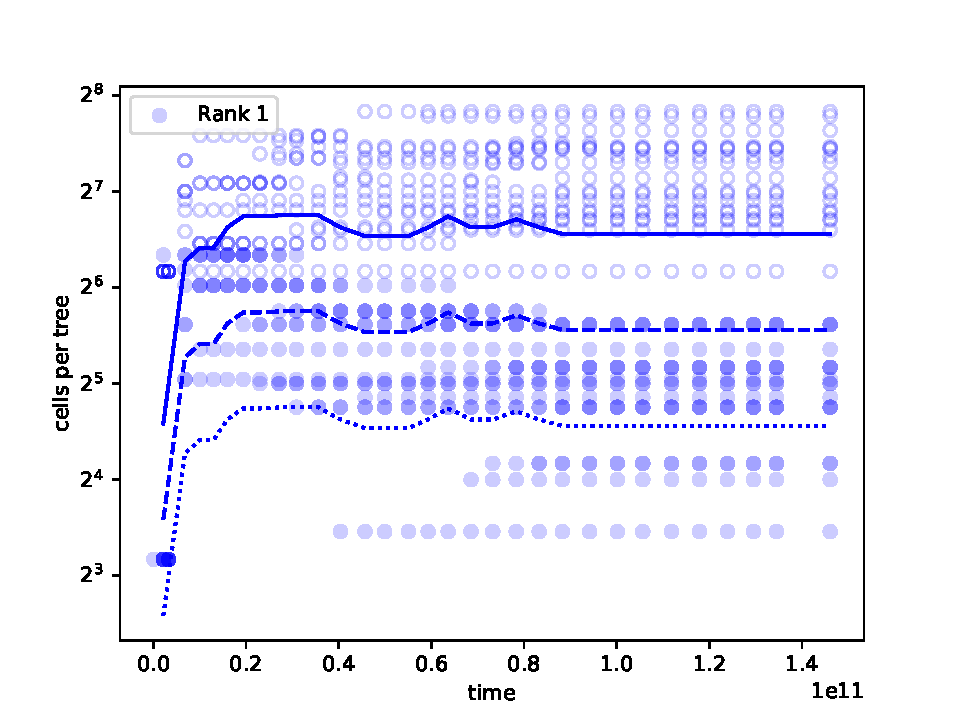
\includegraphics[width=0.7\textwidth]{80_postprocessing/shared-memory.pdf}
\end{center}

\noindent
The script works for shared and distributed memory and gives you a scatter plot
over the load distribution.
Above, you see an (outdated) screenshot of the type of plots---the up-to-date
version should have a legend that is easier to digest.


\paragraph{\ExaHyPE\ postprocessing.}
%
%
%
\ExaHyPE\ has a tailored postprocessing module in its Python API. It yields
graphs alike the one below.
The likely most interesting feature is that it works on archives of data dumps
and thus keeps the disk space usage (and disk accesses) down.


\begin{center}
  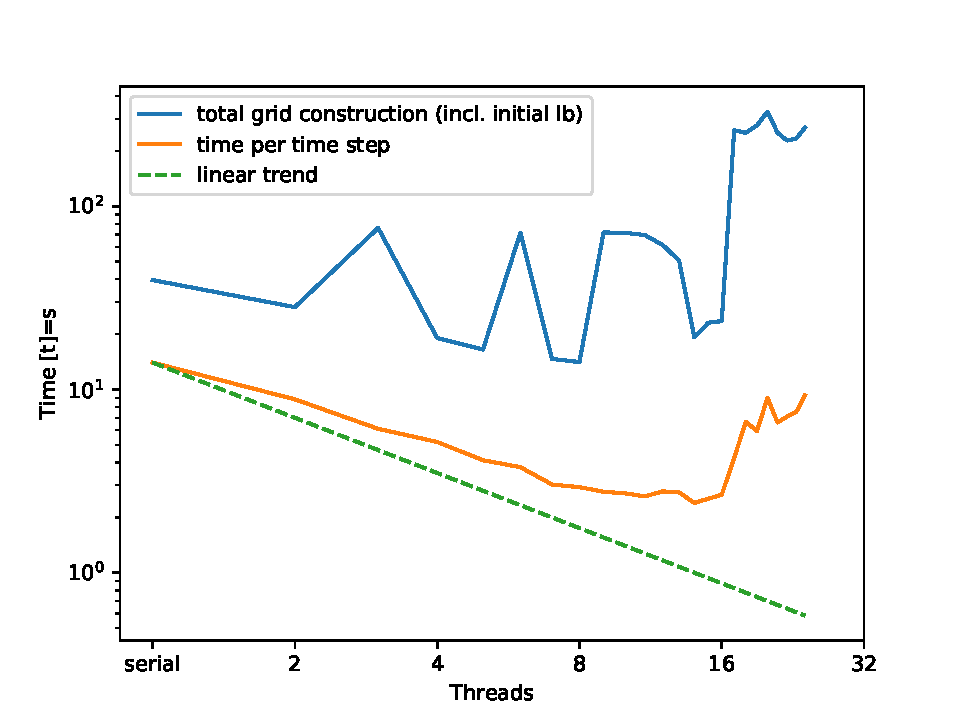
\includegraphics[width=0.7\textwidth]{80_postprocessing/distributed-memory-single-experiment.pdf}
\end{center}

\noindent
There's a couple of parameters to pass to this script to control what exactly is
presented:

\begin{itemize}
  \item Are you interested in both the grid construction and the solution time?
  \item Do you want the script to take the whole simulation time into account or
  only the last time step?
  \item \ldots
\end{itemize}


